%!TEX root = ../report.tex

\begin{document}
	\let\cleardoublepage\clearpage
    \chapter{Background} \label{background}
    This section elaborately discusses the concepts which help the readers to understand the remaining parts of this research work.
    
    \section{Data model}
    
    "A data model is an abstract model that organizes elements of data and standardizes how they relate to one another and to properties of the real world entities. For instance, a data model may specify that the data element representing a car be composed of a number of other elements which, in turn, represent the color and size of the car and define its owner." \cite{misc08}
    
    In Database Management Systems context, a data model depicts the structure of data stored and obtained from the database. Different database systems follow different ways of how they store the data physically in the device, and the users may choose the database based on their application requirements. A good data model determines the overall performance of the application. In Database Management Systems context, data model depicts the structure of data stored and obtained from the database. Different database systems follow different ways of how they store the data physically in the device, and the users may choose the database based on their application requirements. A good data model determines the overall performance of the application. 
    
    \subsection{Types of data models}
     There are many types of data models available. However, some important data models mentioned below are widely approved and utilized in various fields.
    \begin{itemize}
    	\item Relational data model is one of the traditional data models which represents the attributes as column names and the actual data in the form of rows.
    	\item Graph data model is the newcomer in the market and solves many problems in social networking applications. It stores the data as properties in nodes as well as in the edges that connect two different nodes.
    	\item Document data model is the competition for Relational data models since this data model does not stress uses to provide a valid data schema. So, users can store data like documents or semi-structured data. 
    	\item Column family data model stores the data in individual column and columns that fall under the same category can be grouped as a column family.  
    	\item Few databases in the market support a mixture of these existing data models and those databases are called as Multi-model databases.
    \end{itemize}
	
	\section{Database Schema}
	The database schema is a formal language used to define "the blueprint of how a database is constructed" \cite{misc09}. Schema definition differs from database to database and also based on the data model that the database uses. For example, in a relational data model database, schema includes the table, column names, column data types, views, packages, procedures, functions, and relationships. 

	\section{Query Language}
	Query language is a mechanism to read or access the data stored in a database.  All databases provide their own query language implementation to let users execute the query and get results from the database. For example, MongoDB have MongoDB Command Line Interface based on javascript, MySQL have Structured Query Language, Cassandra have Cassandra Query Language.
	
	\section{Federated database}
	
	A federated database system acts as a meta-database management system which "maps different autonomous databases into a single federated database" \cite{misc10}.  Each independent homogeneous databases are located in different places and interconnected through the network connection. Federated database acts as a middle man between these databases regardless of how the data is stored and merge the results from all the databases. Federated databases allow users to use a unique querying platform and execute a single query to read and store the data from various types of databases even though the databases are heterogeneous. Federated database systems divide the single query into subqueries according to the underlying database systems and accumulate the result sets from each subquery and combine them into a single final response.  FDS internally have different types of wrappers to translate the subqueries to appropriate database query language.
	
	In FDBS architecture may consist of centralized or decentralized (distributed) databases where centralized system controls a single database instance, and decentralized system controls multiple dependent/independent database instances. An FDBS can be a nonfederated database system if any one of the databases is non-autonomous in the participating group. So it means that a system can be called as FDBS only if all the participating databases are entirely autonomous and should "allow partial and controlled sharing of their data" \cite{misc10}.
	
	\subsection{Loosely coupled FDBS}
	
	Loosely coupled federated systems define their own schema format that is used by everyone to access the databases involved in the federation. This approach forces the user to learn the federation schema to work with multi-databases.

	\subsection{Tightly coupled FDBS}
	
	Tightly coupled federated systems have separate processes for every database involved in the federation to build and export integrated federated schema.
	
	\subsection{Heterogeneity}
	There are significant factors that cause the heterogeneity in database systems such as semantics, structures, and the query language. 
	Semantic heterogeneities occur if there is a conflict between the meaning of attributes, how it can be interpreted, and how the consumes use the data. There are a few well-known conflicts mentioned below,
	\begin{itemize}
		\item Data representation conflict
		\item Data conflict (missing attributes)
		\item Metadata conflict
		\item Precision conflict
		\item Naming conflict
		\item Schema conflict
	\end{itemize}
	
	Structural heterogeneities happen when there are different primitives between the two data models.
	
	\subsection{Data abstraction}
	Data abstraction in the context of database systems hides crucial complexities through many levels \ref{fig:Data_abstraction_levels}, and it is vital for constructing a federated database system.
	
	\begin{figure}[!htbp] 
		\begin{center}
			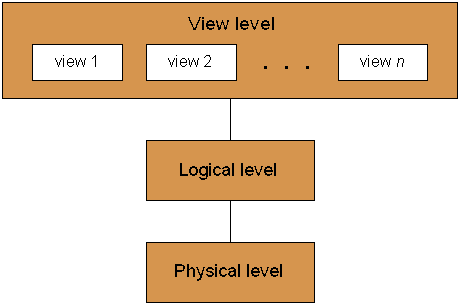
\includegraphics[scale=0.9]{./images/Data_abstraction_levels}	
			\caption{Different layers of data abstraction in database systems \cite{misc12}}	
			\label{fig:Data_abstraction_levels}	
		\end{center}
	\end{figure}
	
	\begin{itemize}
		\item Physical level abstraction is the lowest level of abstraction which handles the data storage in the real systems. 
		\item Logical level abstraction handles the type of data being stored in the database and the relationships between those data.
		\item View level abstraction is the highest level of abstraction which modularizes the big database system into smaller structures because users may not need to access complete information about the database, rather they interest in few parts of the database. 		
	\end{itemize}

 	\section{JSON Schema} \label{sec:json_schema}
	
	JSON Schema is extensively used in this research work for mapping possible sensor input data attributes and types with the GraphQL type definitions. JSON Schema is "a JSON based format for defining the JSON data" \cite{misc13}. It is a complete specification to define the types of each field in the data, restrictions for those fields,  and marks the required fields in the data. A simple example is illustrated in the figure \ref{fig:json_schema} which shows the JSON schema for a piece of robot information. 
	
	\begin{figure}[!htbp] 
		\begin{center}
			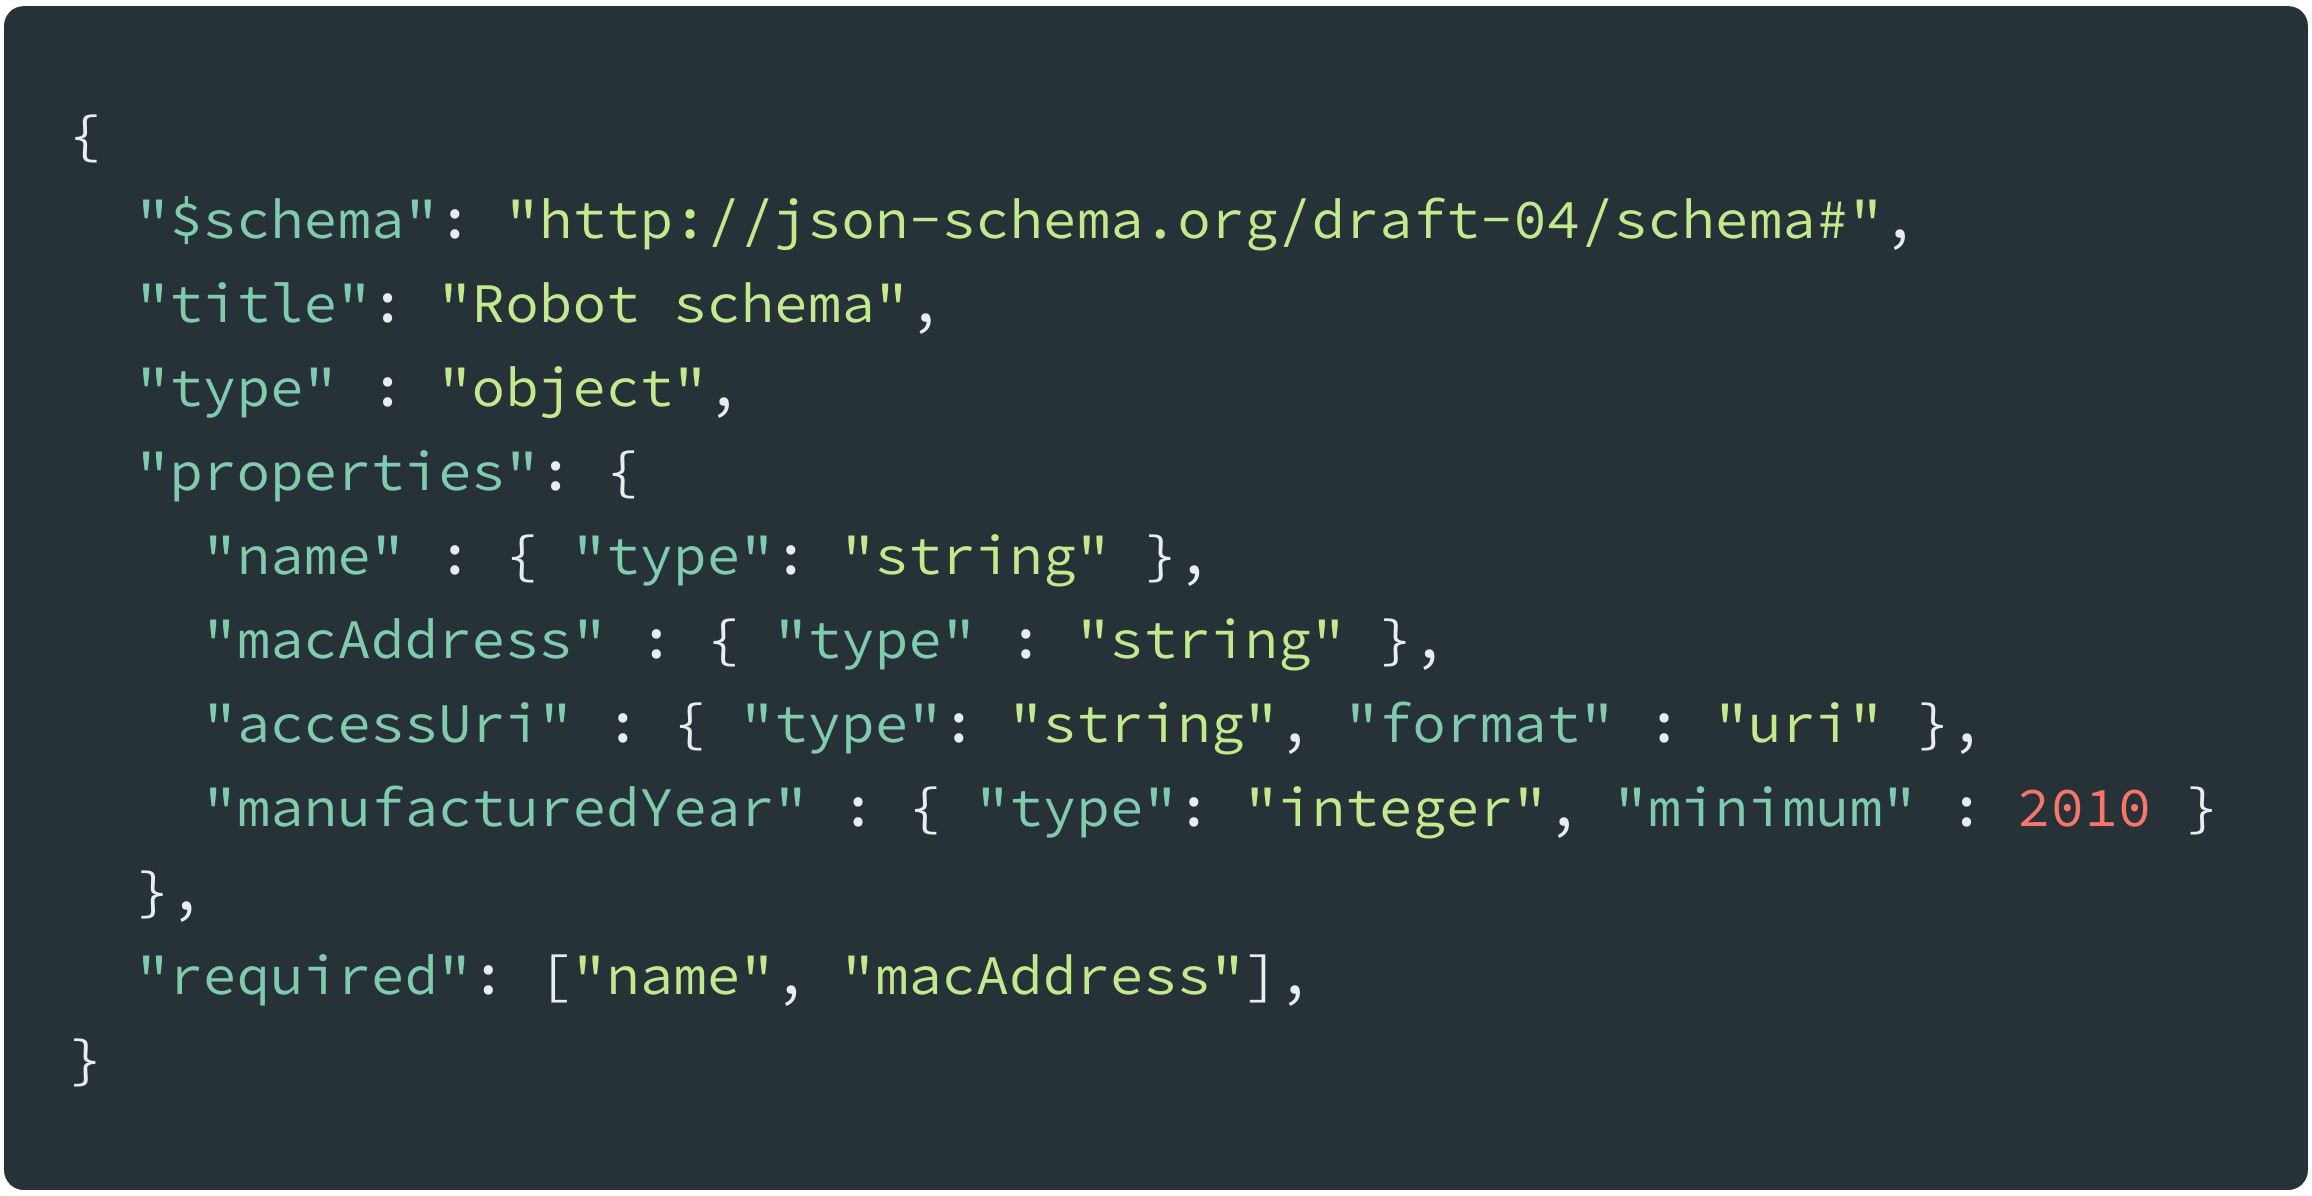
\includegraphics[scale=0.1]{./images/png/json_schema}	
			\caption{Simple JSON Schema represents the properties and constraints of Robot JSON document.}	
			\label{fig:json_schema}	
		\end{center}
	\end{figure}
	
	
	In the JSON Schema document, first attribute '\$schema' defines the JSON schema draft version which is followed to create this document. This attribute helps the consumers or tools to parse the document with appropriate versions. Next, the 'title' attribute defines the title for the JSON schema, 'type' defines the data type of the real JSON data. For example, the given example tells that the robot information will be an 'object'. Then, 'properties' filed holds all the possible attributes of the robot object and their types and format. One can add a constraint on any field in the properties like 'manufacturedYear' property have a constraint of 'minimum' value should be 2010. Also, users can define the format for the value like date, URI, uuid, etc. Finally, the required field indicates the name and macAddress properties are mandatory.
	
	
	\section{@context}
	@context in JSON-LD document used to map the terms to their original context. A term represents a key-value pair in a JSON document. With the help of context, a term can be expanded to a full URL.
	
	\section{Node js}
	
	Node.js is a cross-platform JavaScript run-time environment used to run JavaScript programs without a browser. JavaScript programs are meant to execute in the client side browser's JavaScript engine. NodeJS let the developers write and run JavaScript programs in an isolated environment called node which uses Google's V8 JavaScript engine.  It is used to develop command line tools and server-side scripting, and it overcomes the gap between client and server side programming since traditionally developers use two different languages on client and server side. In our research work, we develop the mediator component as a Node js application for a various good reason, and it will be discussed in the mediator component implementation section.
	
	\section{MongoDB}
	MongoDB is a document database that provides high performance, high availability and automatic scaling. MongoDB stores data in the form of document and it consists of field and value pairs which are similar to JSON objects. The value may include other documents, arrays, and arrays of documents. A set of documents belongs to a collection.
	
	\section{MySQL}
	MySQL is a well-known Relational Database Management System. It stores data in tables and relations can be defined between tables using primary and foreign keys to represent the connection between data. It indexes data based on the primary key which improves the speed of reading query execution. Data model or schema should be defined before inserting data into tables. It provides ACID property to provide strong consistency on the data and it also available depends on the chosen configuration.
	
	\section{Docker}
	"Docker is an open source platform for developing, shipping and running applications" \cite{misc11}. Important components of docker are, images, and containers. Images are nothing but a software package or operating system like Ubuntu, Nginx, etc., Using docker platform, one can quickly combine images and necessary software packages to deploy a container. A container is an isolated component runs individually in the docker engine, and multiple containers can be connected and communicated with each other in the same network. Docker engine shares the host machines resources (CPU, Memory) with the running containers. We can write a new image file on top of other base image file to build our customized containers.
	
	\begin{figure}[!htbp] 
		\begin{center}
			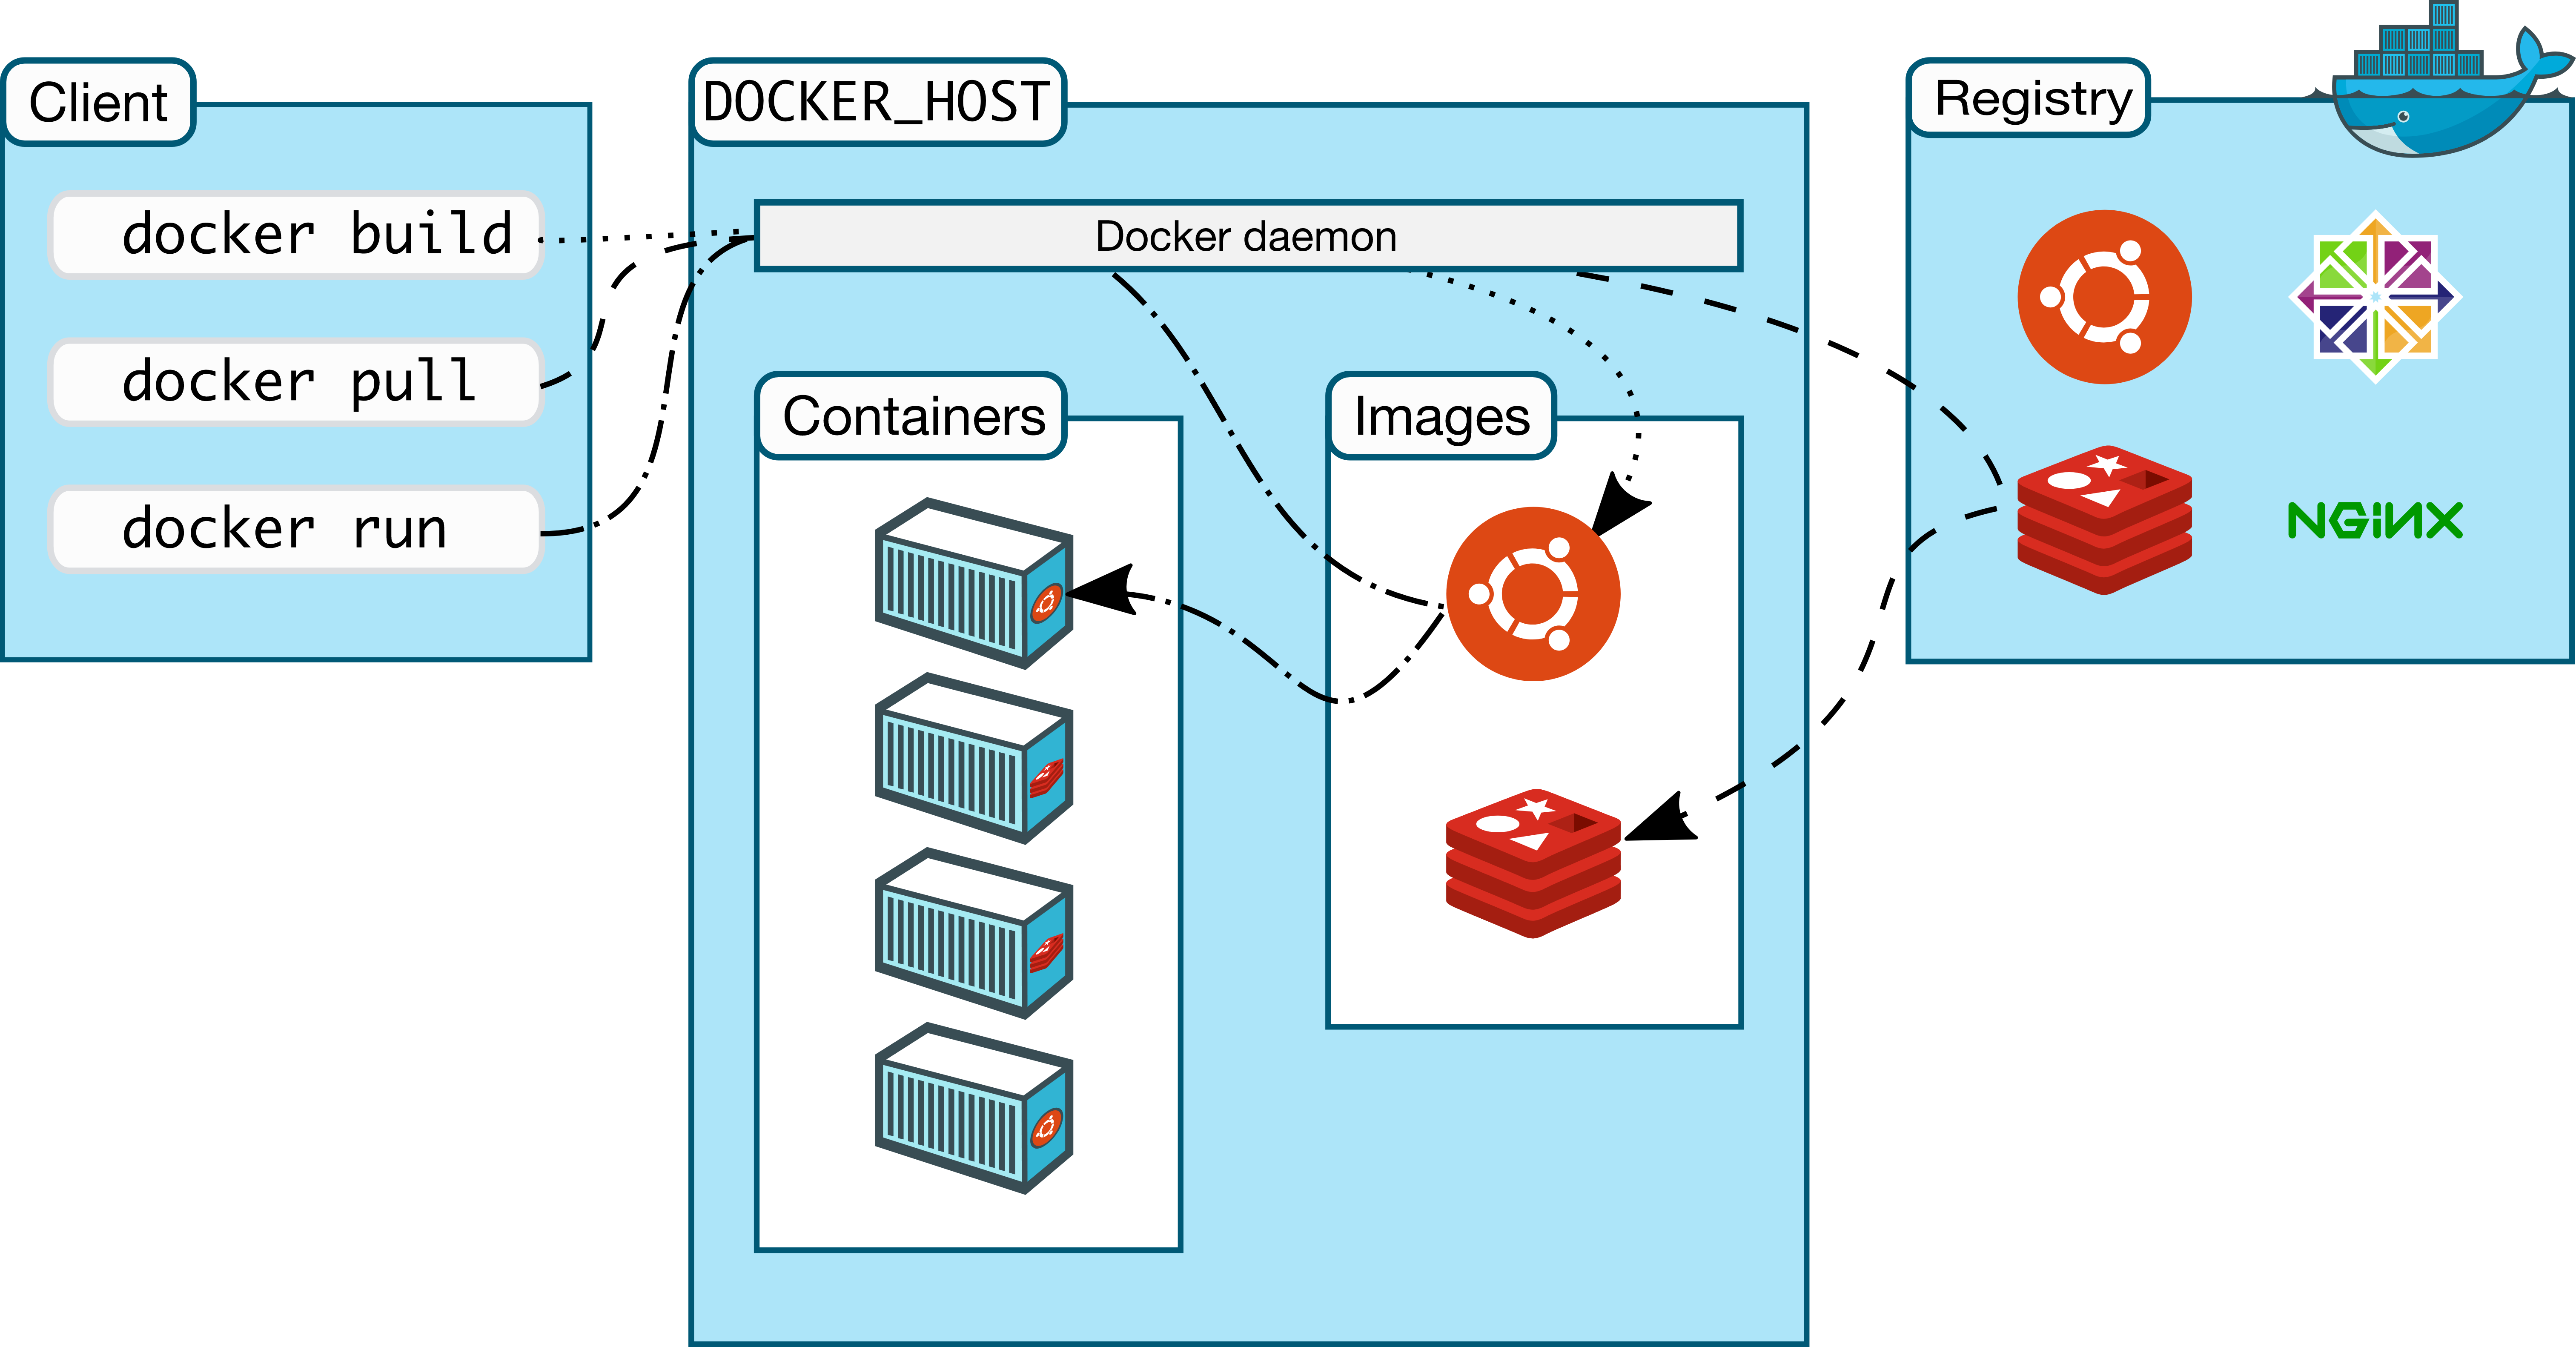
\includegraphics[scale=0.04]{./images/png/docker_architecture}	
			\caption{Docker architecture \cite{misc14}}	
			\label{fig:docker_architecture}	
		\end{center}
	\end{figure}

\end{document}
